\chapter{Analysis}\label{chapter:analysis}

\section{Explanation of $\mathbf{\alpha}$--Parametrized Behavior}\label{section:explanation}

\PARstart{I}{ncluding} the $\alpha_i$ parameter in the Generalized CU constraints, given in equation \ref{eqn:gcu},
creates an asymptotic scale on which the terms $\m{M}_i$ and $(\v{u}-\v{m}_i)$ are balanced. At the two extremes are the
following cases:
\begin{enumerate}
\item If $\m{M}_i$ is a zero matrix, $\alpha_i$ is allowed to approach 0 as well, and the constraint reduces to
$\m{U}\geq (\v{u}-\v{m}_i)(\v{u}-\v{m}_i)^T$, and
\item If $\v{u}$ and $\v{m}_i$ are coincident, $\alpha_i$ is allowed to approach 1, and the constraint reduces to
$\m{U}\geq \m{M}_i$.
\end{enumerate}
For the general case, in which both terms are nonzero, the actual value of $\alpha_i$ will be bounded somewhere between
0 and 1. It is not important to know this actual value, since it is determined by the optimization process in
conjunction with the other $n-1$ estimates.

With this knowledge, it is possible to logically reduce the question of whether Generalized CU and MEEE are equivalent.
First, since it is necessary to satisfy all $n$ constraints in equation \ref{eqn:gcu}, a minimal L\"owner
ellipsoid $\varepsilon_0$ for $(\v{u},\m{U})$ will be one that completely contains the ellipsoid $\varepsilon_i$ for
each $(\v{m}_i,\m{M}_i)$ in $i=1\dots n$~\cite{yildirim06}. Second, if the ellipsoid $\tau_i$ for
$(\v{u},\frac{\m{M}_i}{\alpha_i}+\frac{(\v{u}-\v{m}_i)(\v{u}-\v{m}_i)^T}{1-\alpha_i})$ completely contains
$\varepsilon_i$, it follows that $\varepsilon_0$ will completely contain $\varepsilon_i$ as well, since $\tau_i$ and
$\varepsilon_0$ are both centered at $\v{u}$ and $\varepsilon_0$ is at least as large as $\tau_i$. Therefore, if
$\tau_i$ can be shown to completely enclose $\varepsilon_i$ for all values of $\alpha_i\in (0,1)$, for
all $i=1\dots n$, then $\varepsilon_0$ is a L\"owner ellipsoid, and Generalized CU and MEEE are in fact equivalent.

Formally, $\varepsilon_i$ and $\tau_i$ are the 1-$\sigma$ ellipsoids transformed by equation \ref{eqn:cu2e}; of
\begin{align}
    \displaystyle
    \varepsilon_i    &= \mathbb{T}\left(\v{m}_i,\m{M}_i\right)\label{eqn:coveps}\\
    \tau_i(\alpha_i) &=
\mathbb{T}\left(\v{u},\frac{\m{M}_i}{\alpha_i}+\frac{(\v{u}-\v{m}_i)(\v{u}-\v{m}_i)^T}{1-\alpha_i}\right)\label{eqn:covtau}
\end{align}
The containing ellipsoid $\tau_i$ varies with $\alpha_i$, with all other terms constant. An analysis of this behavior
follows.


% 1D
\section{Describing the Behavior in One Dimension}

Since the 1-$\sigma$ ellipsoid of a Gaussian curve in one variable is a line, the mathematics are extremely simple; it
becomes extremely easy to visualize and plot the data, and to check the results by hand. Notationally,
$(\v{m}_i,\m{M}_i)$ is just $(\mu_i,\sigma_i^2)$, and the PDF of the estimate is given by the unweighted Gaussian
function
\begin{equation}\label{eqn:gauss1d}
    \varphi_{\mu_i,\sigma_i^2}(x)=e^\frac{-(\mu_i-x)^2}{2\sigma_i^2}, \end{equation}
and the 1-$\sigma$ ellipsoid is the band between $\mu_i-1\sigma_i$ and $\mu_i+1\sigma_i$. The $y$ value of the
1-$\sigma$ line is $\varphi_{\mu_i,\sigma_i^2}(x=\mu_i\pm\sigma_i)=e^{-\frac{1}{2}}\approx0.6065$.

% EXAMPLE 1D CU
\begin{example}[Generalized CU in One Dimension]\label{ex:gcu1d}

Consider a set of four estimates $(\mu_i,\sigma_i^2)$, given by
\begin{figure}[tbp]
    \centering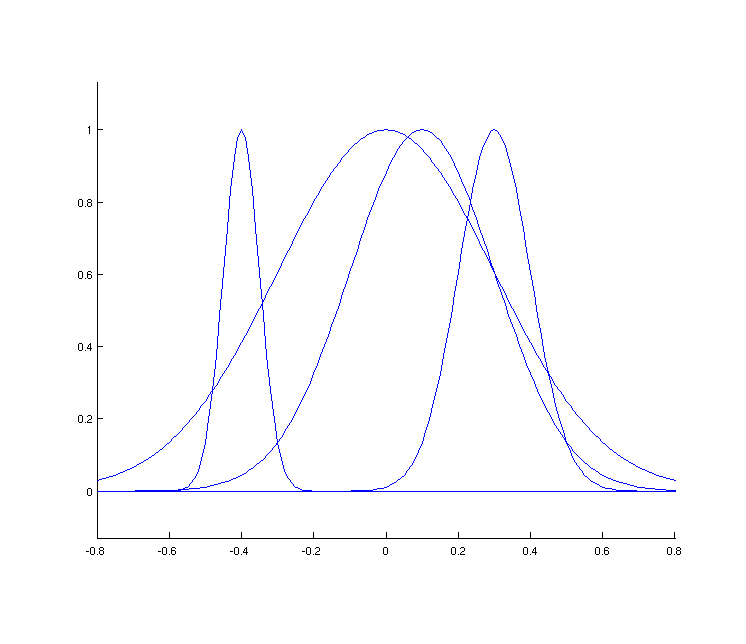
\includegraphics[width=0.6\textwidth]{figures/est1d-4.png}
    \caption{\it 1D Gaussian curves for four estimate means and covariances, for example \ref{ex:gcu1d}.}
    \label{fig:est1d-4}
\end{figure}
\begin{align}
    (\mu_1,\sigma_1^2) &= (0.3000,0.1000^2)\\\nonumber
    (\mu_2,\sigma_2^2) &= (0.1000,0.2000^2)\\\nonumber
    (\mu_3,\sigma_3^2) &= (0.0000,0.3000^2)\\\nonumber
    (\mu_4,\sigma_4^2) &= (-0.4000,0.0500^2),\label{ex:est1d-4}
\end{align}
shown in figure \ref{fig:est1d-4}. Applying batch Generalized CU to these inputs,
\begin{equation}
    (\mu_u,\sigma_u^2) = \GCU\left((\mu_1,\sigma_1^2),(\mu_2,\sigma_2^2),(\mu_3,\sigma_3^2),(\mu_4,\sigma_4^2)\right)
\end{equation}
yields the values
\begin{figure}[tbp]
    \centering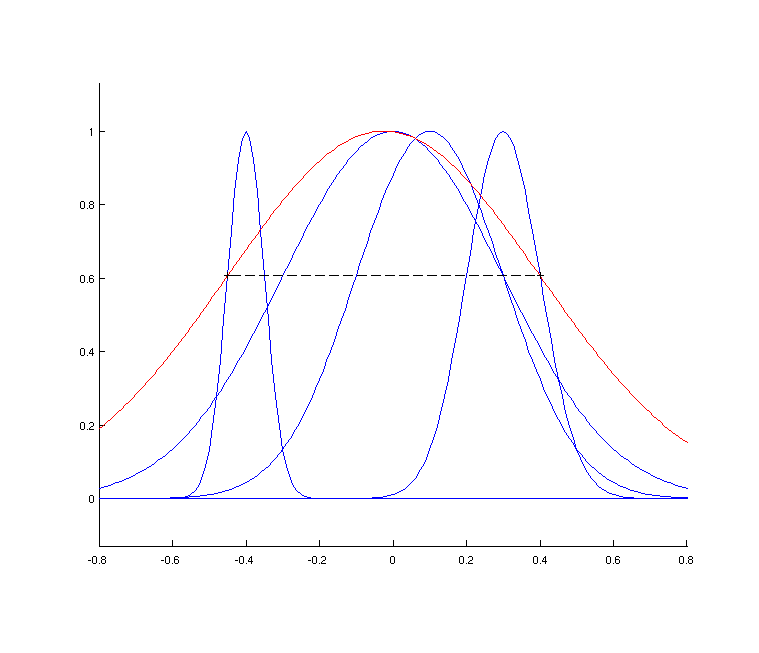
\includegraphics[width=0.6\textwidth]{figures/cu1d.png}
    \caption{\it 1D Gaussian curves for four inputs (blue), together with the batch Generalized CU result (red) and
            its 1-$\sigma$ ellipsoid (dashed), for example \ref{ex:gcu1d}.}
    \label{fig:cu1d}
\end{figure}
\begin{equation}
    (\mu_u,\sigma_u^2) = (-0.0250,0.4250^2).
\end{equation}
Figure \ref{fig:cu1d} shows the inputs plotted with the Gaussian curve for $(\mu_u,\sigma_u^2)$. The 1-$\sigma$ line,
from $x=\mu_u-\sigma_u$ to $x=\mu_u+\sigma_u$, at $y=e^{-\frac{1}{2}}$, corresponds to the outermost intersection points
between the inputs and the CU result curves. The boundary points for each 1-$\sigma$ ellipsoid are $x=\mu_i\pm\sigma_i$:
\begin{align}
    \mu_1-\sigma_1 &= 0.2000 & \mu_1+\sigma_1 &= 0.4000\nonumber\\
    \mu_2-\sigma_2 &= -0.1000 & \mu_2+\sigma_2 &= 0.3000\nonumber\\
    \mu_3-\sigma_3 &= -0.3000 & \mu_3+\sigma_3 &= 0.3000\nonumber\\
    \mu_4-\sigma_4 &= -0.4500 & \mu_4+\sigma_4 &= -0.3500\\
\intertext{Of these points, $\mu_4-\sigma_4$ and $\mu_1+\sigma_1$ exactly equal the 1-$\sigma$ points on the CU curve,}
    \mu_u-\sigma_u &= -0.4500 & \mu_u+\sigma_u &= 0.4000,
\end{align}
and the remaining points are all within the range $(-0.4500,0.4000)$.

Following the logic outlined in section \ref{section:explanation}, it is
necessary to consider the ellipsoid $\varepsilon_1$ from equation \ref{eqn:coveps} and $\tau_1(\alpha_1)$ from equation
\ref{eqn:covtau}:
\begin{align}
    \varepsilon_1 &= \mathbb{T}\left(\mu_1,\sigma_1^2\right) = \mathbb{T}\left(0.3000,0.0100\right)\\
    \tau_1(\alpha_1) &= \mathbb{T}\left(\mu_u,\frac{\sigma_1^2}{\alpha_1}+\frac{(\mu_u-\mu_1)^2}{1-\alpha_1}\right)
        = \mathbb{T}\left(-0.0250,\frac{0.0100}{\alpha_1}+\frac{0.1056}{1-\alpha_1}\right).
\end{align}
From equation \ref{eqn:cu2e}, the transformation into ellipsoid space is:
\begin{align}
    \varepsilon_1 &= \left\{
        \begin{aligned}
            A_{\varepsilon,1} &= 100\\
            b_{\varepsilon,1} &= -30\\
            c_{\varepsilon,1} &= 8
        \end{aligned}\right.,\\\nonumber
    \tau_1(\alpha_1) &= \left\{
        \begin{aligned}
            A_{\tau,1} &= \frac{\begin{smallmatrix}1\end{smallmatrix}}{\frac{0.0100}{\alpha_1}+\frac{0.1056}{1-\alpha_1}} \\
            b_{\tau,1} &= \frac{\begin{smallmatrix}0.0250\end{smallmatrix}}{\frac{0.0100}{\alpha_1}+\frac{0.1056}{1-\alpha_1}} \\
            c_{\tau,1} &= \frac{\begin{smallmatrix}0.0062\end{smallmatrix}}{\frac{0.0100}{\alpha_1}+\frac{0.1056}{1-\alpha_1}} -1 \\
        \end{aligned}\right.
\end{align}
Equation \ref{eqn:ellipse} (repeated here)
\begin{equation}
    \varepsilon_i = \{ x | x^TA_ix + 2b_i^Tx + c_i \leq 0 \}\nonumber
\end{equation}
gives the quadratic formulation for an $n$-dimensional ellipsoid. In one dimension, $\varepsilon_1$ can be written as
\begin{equation}
    \varepsilon_1 = 100x^2-60x+8 \leq 0,
\end{equation}
and solving for the roots gives
\begin{equation}
    x = 0.2, \qquad x = 0.4,
\end{equation}
which are exactly equal to $\mu_1\pm\sigma_1$. For $\tau_1(\alpha_1)$ to completely contain $\varepsilon_1$, its roots
must bound the roots of $\varepsilon_1$ for all values of $\alpha_1\in(0,1)$.
\begin{figure}[tbp]
    \centering
        \subfloat[$\alpha_1$=0.05]{\label{fig:alpha1d05}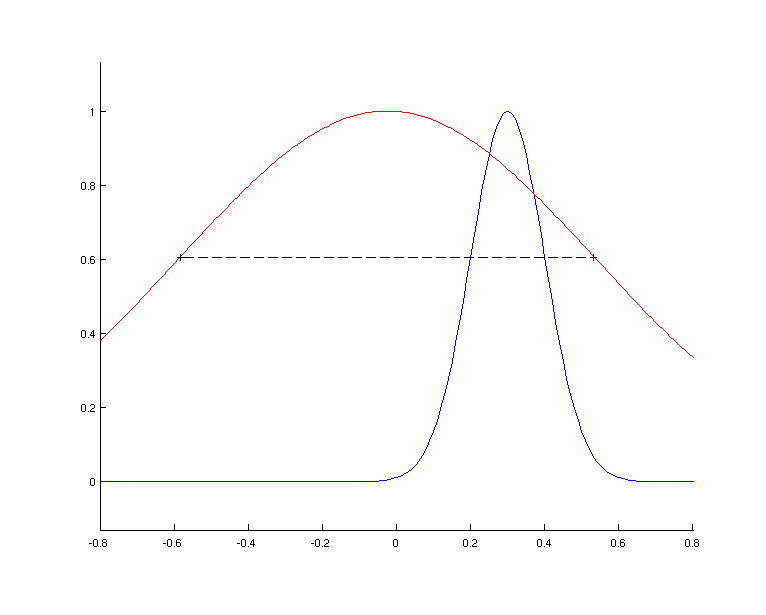
\includegraphics[width=0.4\textwidth]{figures/alpha1d-05.png}}
        \subfloat[$\alpha_1$=0.25]{\label{fig:alpha1d25}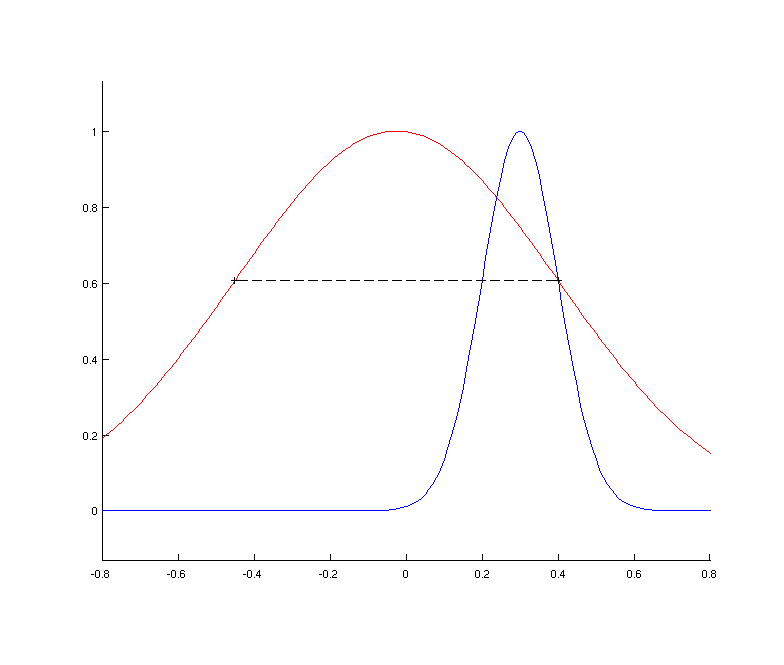
\includegraphics[width=0.4\textwidth]{figures/alpha1d-25.png}}

        \subfloat[$\alpha_1$=0.50]{\label{fig:alpha1d50}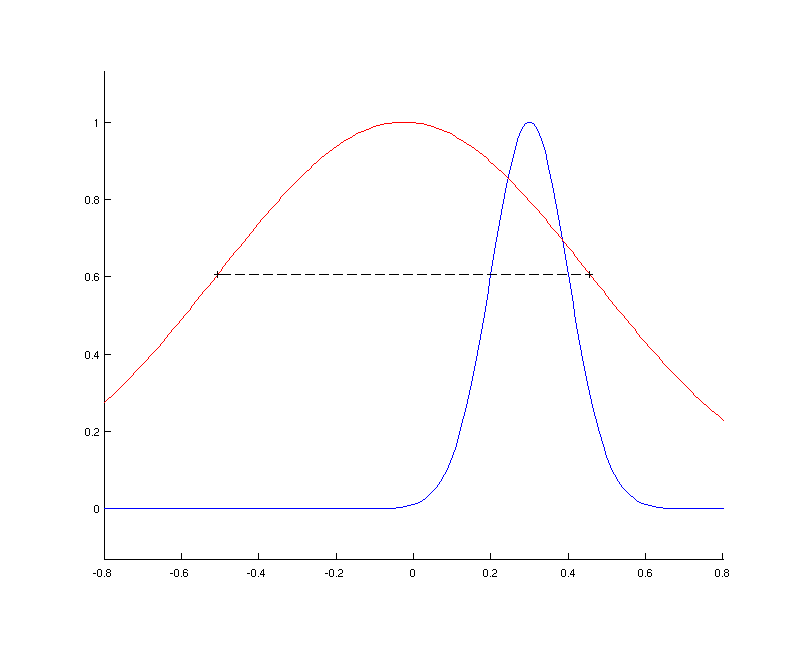
\includegraphics[width=0.4\textwidth]{figures/alpha1d-50.png}}
        \subfloat[$\alpha_1$=0.75]{\label{fig:alpha1d75}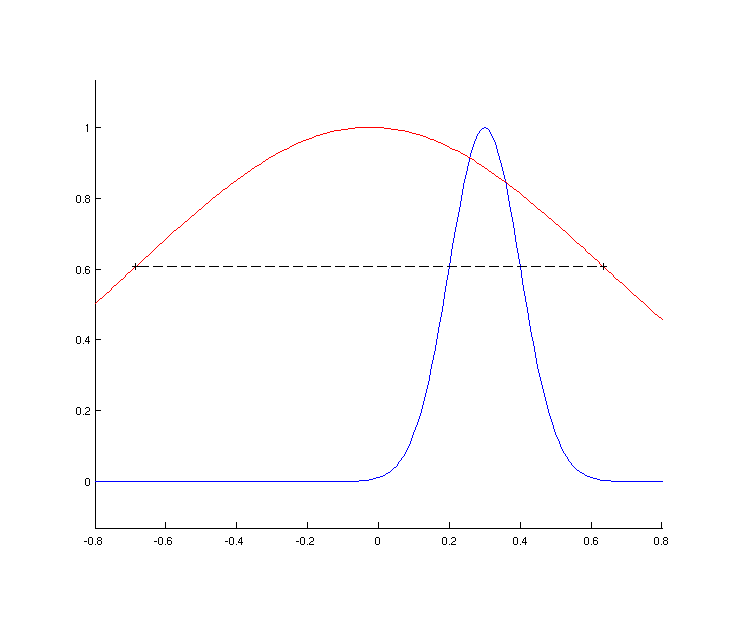
\includegraphics[width=0.4\textwidth]{figures/alpha1d-75.png}}

        \subfloat[$\alpha_1$=0.95]{\label{fig:alpha1d95}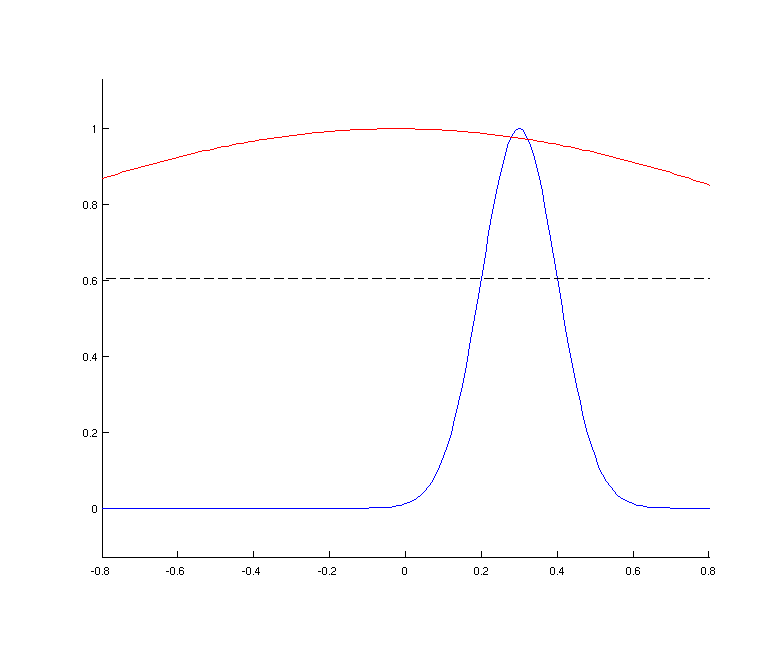
\includegraphics[width=0.4\textwidth]{figures/alpha1d-95.png}}
    \caption{\it 1D Gaussian curves for estimate $(\v{m}_1,\m{M}_1)$ and the intermediate error covariance (red), and
            its 1D 1-$\sigma$ ellipsoid (dashed), for example \ref{ex:gcu1d}.}
    \label{fig:alpha1d}
\end{figure}
By choosing a value for $\alpha_1$, it is possible to numerically determine the intermediate error covariance
$\left(\mu_u,\frac{\sigma_1^2}{\alpha_1}+\frac{(\mu_u-\mu_1)^2}{1-\alpha_1}\right)$, and the 1-$\sigma$ ellipsoid
$\tau_1(\alpha_1)$ and its roots. Using the ellipsoid transformation (equation \ref{eqn:cu2e}) and quadratic ellipsoid
equation (\ref{eqn:ellipse}) as above, the roots of $\tau_1(\alpha_1)$ are:
\begin{equation}
    x = \begin{cases}
            -0.5828, 0.5328 \qquad \text{for $\alpha_1 = 0.05$}\\
            -0.4502, 0.4002 \qquad \text{for $\alpha_1 = 0.25$}\\
            -0.5059, 0.4559 \qquad \text{for $\alpha_1 = 0.50$}\\
            -0.6852, 0.6352 \qquad \text{for $\alpha_1 = 0.75$}\\
            -1.4821, 1.4321 \qquad \text{for $\alpha_1 = 0.95$}
        \end{cases}
\end{equation}
\begin{figure}[tbp]
    \centering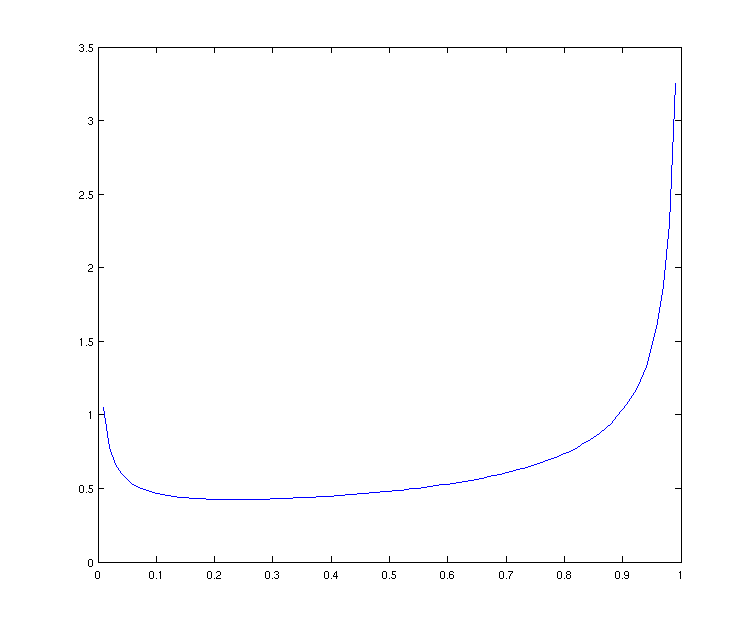
\includegraphics[width=0.6\textwidth]{figures/alpha1dcurve.png}
    \caption{\it $\alpha_1$ vs $\sigma_{intermediate,1}$ for example \ref{ex:gcu1d}.}
    \label{fig:alpha1dcurve}
\end{figure}
Since the roots of $\tau_1(\alpha_1)$ can also be written as $\mu_u\pm\sigma_{intermediate,1}$, it is also useful to
find the value of the intermediate standard deviation
\begin{equation}
    \sigma_{intermediate,1} = \sqrt{\frac{\sigma_1^2}{\alpha_1}+\frac{(\mu_u-\mu_1)^2}{1-\alpha_1}}
\end{equation}
and plot it versus $\alpha_1$, as shown in figure \ref{fig:alpha1dcurve}. The minimum value for
$\sigma_{intermediate,1}$ occurs at $\alpha_1=0.2350$, so the smallest ellipsoid $\tau_1(\alpha_1)$ is:
\begin{equation}
    \tau_1(\alpha_1=0.2350) = \left\{
        \begin{aligned}
            A_{\varepsilon,1} &= 5.5373\\
            b_{\varepsilon,1} &= 0.1384\\
            c_{\varepsilon,1} &= -0.9654
        \end{aligned}\right.
\end{equation}
The quadratic form is
\begin{equation}
    \varepsilon_1 = 5.5373x^2+2768x-0.9654 \leq 0,
\end{equation}
and solving for the roots gives
\begin{equation}
    x = -0.4499, \qquad x = 0.3999,
\end{equation}
which are within acceptable floating-point rounding error of $\mu_u\pm\sigma_{intermediate,1}$.

This procedure can be repeated for $(\mu_2,\sigma_2^2)$, $(\mu_3,\sigma_3^2)$, and $(\mu_4,\sigma_4^2)$ to confirm the
same behavior. The fact that the roots of $\varepsilon_i$ are bounded by the roots of $\tau_i(\alpha_i)$ for all
$\alpha_i\in(0,1)$ implies that $\varepsilon_0 = \mathbb{T}\left(\mu_u,\sigma_u^2\right)$ completely contains each
$\varepsilon_i$, and is therefore a minimal L\"owner ellipsoid.

\end{example}

% 2D
\section{Describing the Behavior in Two Dimensions}

In two dimensions, relative positions between estimate means become more complex, and additionally rotations must be
considered for each covariance body. Regarding notation, $\v{m}_i$ is
$\left[\begin{smallmatrix}\mu_{x,i}\\\mu_{y,i}\end{smallmatrix}\right]$ and $\m{M}_i$ is at least as large as
$\left[\begin{smallmatrix}\sigma_{x,i}\\\sigma_{y,i}\end{smallmatrix}\right]
 \left[\begin{smallmatrix}\sigma_{x,i}&\sigma_{y,i}\end{smallmatrix}\right]$, though $\sigma_{x,i}$ and $\sigma_{y,i}$
may be rotated by any arbitrary amount. The PDF of the estimate is given by the unweighted Gaussian function
\begin{equation}\label{eqn:gauss2d}
    \varphi_{(\mu_{x,i},\mu_{y,i}),(\sigma_{x,i},\sigma_{y,i})} = 
        e^{-\left(\frac{(\mu_{x,i}-x)^2}{2\sigma_{x,i}^2}\right)-\left(\frac{(\mu_{y,i}-y)^2}{2\sigma_{y,i}^2}\right)},
\end{equation}
and the 1-$\sigma$ ellipsoid is a two dimensional ellipse centered at $(\mu_{x,i},\mu_{y,i})$ with axes of length
$2\sigma_{x,i}$ and $2\sigma_{y,i}$, rotated to match $\varphi_{(\mu_{x,i},\mu_{y,i}),(\sigma_{x,i},\sigma_{y,i})}$. The
behavior of the $\alpha$--parametrized intermediate covariance is also more complex, since it is a linear combination
of both the shape of $\m{M}_i$ and the relative distance between the means $\v{m}_i$ and $\v{u}$.


% EXAMPLE 2D CU
\begin{example}[Generalized CU in Two Dimensions]\label{ex:gcu2d}

Consider as set of four estimates $(\v{m}_i,\m{M}_i)$, given by
\begin{figure}[tbp]
    \centering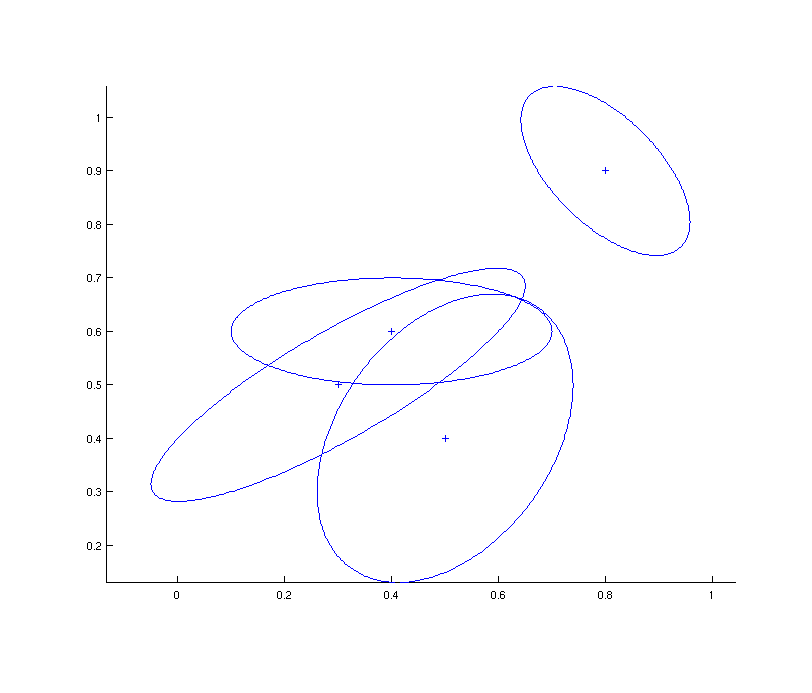
\includegraphics[width=0.6\textwidth]{figures/est2d-4.png}
    \caption{\it 1-$\sigma$ contour ellipsoids for four 2D input estimate means and covariances used in example \ref{ex:gcu2d}.}
    \label{fig:est2d-4}
\end{figure}
\begin{align}
    (\v{m}_1,\m{M}_1) &= \left(\left[
        \begin{smallmatrix}
            0.3000\\
            0.5000
        \end{smallmatrix}\right],
        \left[
        \begin{smallmatrix}
            0.1225 &  0.0650\\
            0.0650 &  0.0475
        \end{smallmatrix}\right]\right)\nonumber\\
    (\v{m}_2,\m{M}_2) &= \left(\left[
        \begin{smallmatrix}
            0.4000\\
            0.6000
        \end{smallmatrix}\right],
        \left[
        \begin{smallmatrix}
            0.0900 &  0.0000\\
            0.0000 &  0.0100
        \end{smallmatrix}\right]\right)\nonumber\\
    (\v{m}_3,\m{M}_3) &= \left(\left[
        \begin{smallmatrix}
            0.8000\\
            0.9000
        \end{smallmatrix}\right],
        \left[
        \begin{smallmatrix}
            0.0250 & -0.0150\\
           -0.0150 &  0.0250
        \end{smallmatrix}\right]\right)\nonumber\\
    (\v{m}_4,\m{M}_4) &= \left(\left[
        \begin{smallmatrix}
            0.5000\\
            0.4000
        \end{smallmatrix}\right],
        \left[
        \begin{smallmatrix}
            0.0573 &  0.0238\\
            0.0238 &  0.0727
        \end{smallmatrix}\right]\right)
\end{align}
shown in figure \ref{fig:est2d-4}. Applying batch GCU to these inputs,
\begin{equation}
    (\v{u},\m{U}) = \GCU\left((\v{m}_1,\m{M}_1),(\v{m}_2,\m{M}_2),(\v{m}_3,\m{M}_3),(\v{m}_4,\m{M}_4)\right),
\end{equation}
yields the values
\begin{figure}[tbp]
    \centering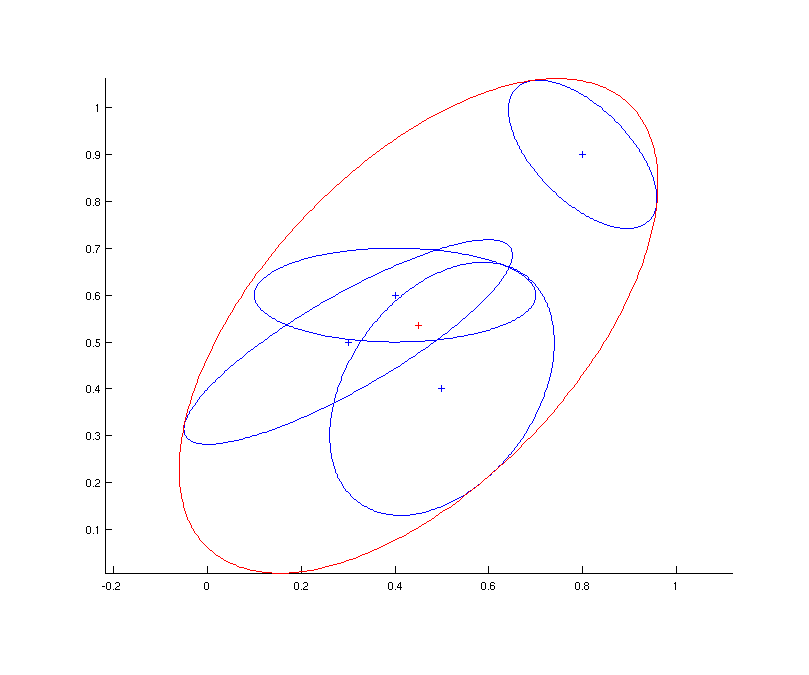
\includegraphics[width=0.6\textwidth]{figures/cu2d-4.png}
    \caption{\it 1-$\sigma$ contour ellipsoids for four inputs (blue) together with the batch Generalized CU result
        (red) for example \ref{ex:gcu2d}.}
    \label{fig:cu2d-4}
\end{figure}
\begin{equation}
    (\v{u},\m{U}) = \left(\left[
        \begin{smallmatrix}
            0.4499\\
            0.5342
        \end{smallmatrix}\right],
        \left[
        \begin{smallmatrix}
            0.2606 &  0.1559\\
            0.1559 &  0.2778
        \end{smallmatrix}\right]\right)
\end{equation}




It is next necessary to consider the ellipsoid $\varepsilon_1$ from equation
\ref{eqn:coveps} and $\tau_1(\alpha_1)$ from equation \ref{eqn:covtau}:
\begin{align}
    \varepsilon_1 &= \mathbb{T}\left(\v{m}_1,\m{M}_1\right) =
        \mathbb{T}\left(\left[\begin{smallmatrix}0.3000\\0.5000\end{smallmatrix}\right],
            \left[\begin{smallmatrix}0.1224 & 0.0650\\0.0650&0.0475\end{smallmatrix}\right]\right)\\
    \tau_1(\alpha_1) &= \mathbb{T}\left(\v{u},\frac{\m{M}_1}{\alpha_1}+\frac{(\v{u}-\v{m}_1)(\v{u}-\v{m}_1)'}{1-\alpha_1}\right)\\
        &= \mathbb{T}\left(\left[\begin{smallmatrix}0.4499\\0.5342\end{smallmatrix}\right],
        \frac{\left[\begin{smallmatrix}0.1225&0.0650\\0.0650&0.0475\end{smallmatrix}\right]}{\alpha_1}+
        \frac{\left[\begin{smallmatrix}0.0225&0.0051\\0.0051&0.0012\end{smallmatrix}\right]}{1-\alpha_1}\right).
\end{align}
From equation \ref{eqn:cu2e}, the transformation into ellipsoid space is:
\begin{align}
    \varepsilon_1 &= \left\{
        \begin{aligned}
            A_{\varepsilon,1} &= \left[\begin{smallmatrix}29.6875& -40.5949\\ -40.5949& 76.5625\end{smallmatrix}\right]\\
            b_{\varepsilon,1} &= \left[\begin{smallmatrix}11.3912\\-26.1028\end{smallmatrix}\right]\\
            c_{\varepsilon,1} &= \begin{smallmatrix}9.6340\end{smallmatrix}
        \end{aligned}\right.,\\\nonumber
    \tau_1(\alpha_1) &= \left\{
        \begin{aligned}
            A_{\tau,1} &= \left({\frac{\left[\begin{smallmatrix}0.1224 & 0.0650\\0.0650& 0.0475\end{smallmatrix}\right]}{\alpha_1}
                                  +\frac{\left[\begin{smallmatrix}0.0225 & 0.0051\\0.0051& 0.0012\end{smallmatrix}\right]}{1-\alpha_1}}\right)^{-1} \\
            b_{\tau,1} &= -\left({\frac{\left[\begin{smallmatrix}0.1224 & 0.0650\\0.0650& 0.0475\end{smallmatrix}\right]}{\alpha_1}
                                  +\frac{\left[\begin{smallmatrix}0.0225 & 0.0051\\0.0051& 0.0012\end{smallmatrix}\right]}{1-\alpha_1}}\right)^{-1} 
                          \left[\begin{smallmatrix}0.3\\0.5\end{smallmatrix}\right]\\
            c_{\tau,1} &= \left[\begin{smallmatrix}0.3&0.5\end{smallmatrix}\right] 
                            \left({\frac{\left[\begin{smallmatrix}0.1224 & 0.0650\\0.0650& 0.0475\end{smallmatrix}\right]}{\alpha_1}
                                  +\frac{\left[\begin{smallmatrix}0.0225 & 0.0051\\0.0051& 0.0012\end{smallmatrix}\right]}{1-\alpha_1}}\right)^{-1} 
                          \left[\begin{smallmatrix}0.3\\0.5\end{smallmatrix}\right] -1\\
        \end{aligned}\right.
\end{align}

\begin{figure}[tbp]
    \centering
        \subfloat[$\alpha_1$=0.05]{\label{fig:alpha2d05}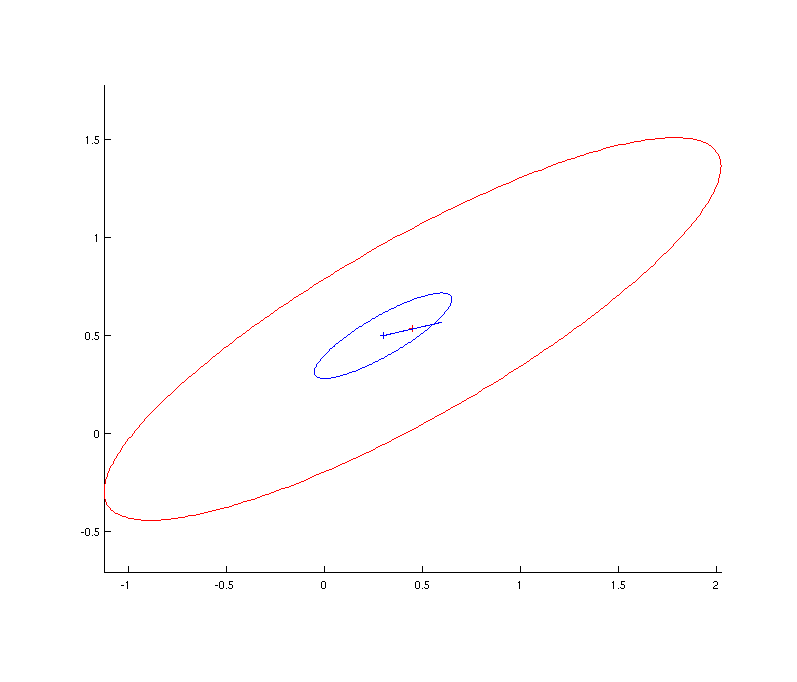
\includegraphics[width=0.4\textwidth]{figures/alpha2d-05.png}}
        \subfloat[$\alpha_1$=0.25]{\label{fig:alpha2d25}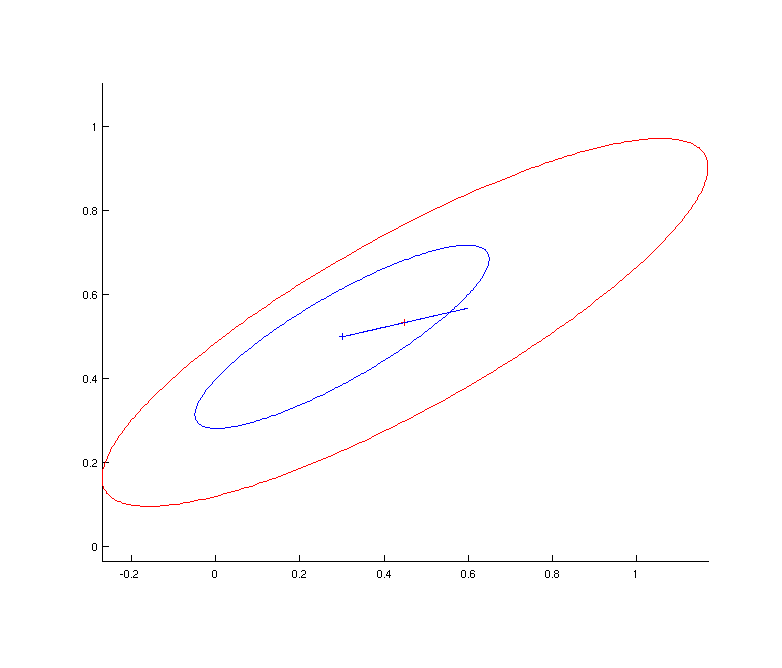
\includegraphics[width=0.4\textwidth]{figures/alpha2d-25.png}}

        \subfloat[$\alpha_1$=0.50]{\label{fig:alpha2d50}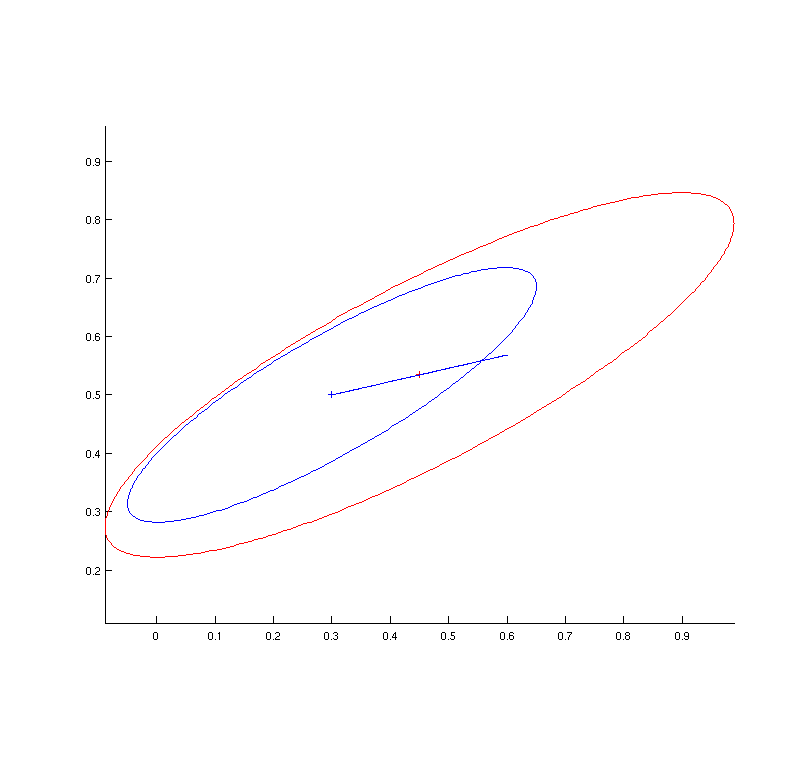
\includegraphics[width=0.4\textwidth]{figures/alpha2d-50.png}}
        \subfloat[$\alpha_1$=0.75]{\label{fig:alpha2d75}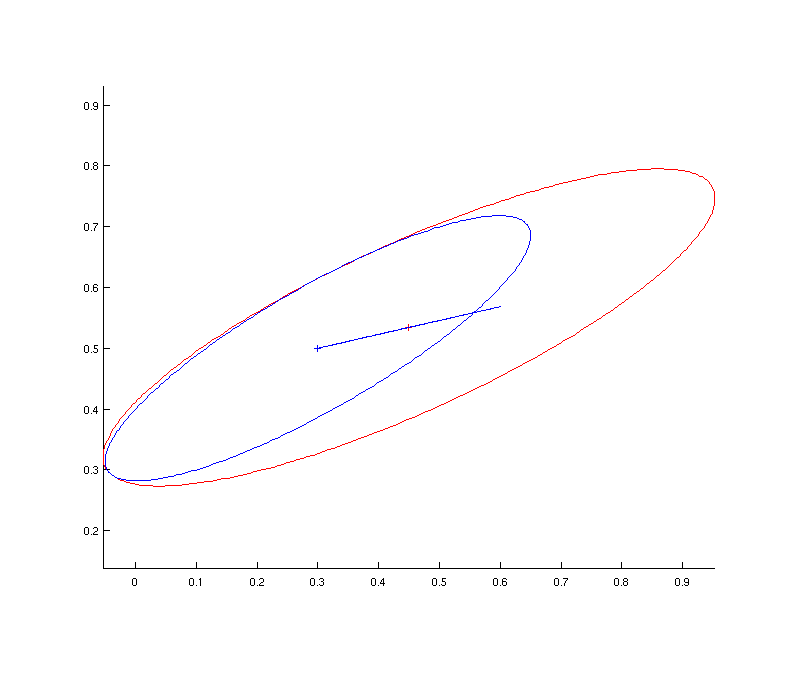
\includegraphics[width=0.4\textwidth]{figures/alpha2d-75.png}}

        \subfloat[$\alpha_1$=0.95]{\label{fig:alpha2d95}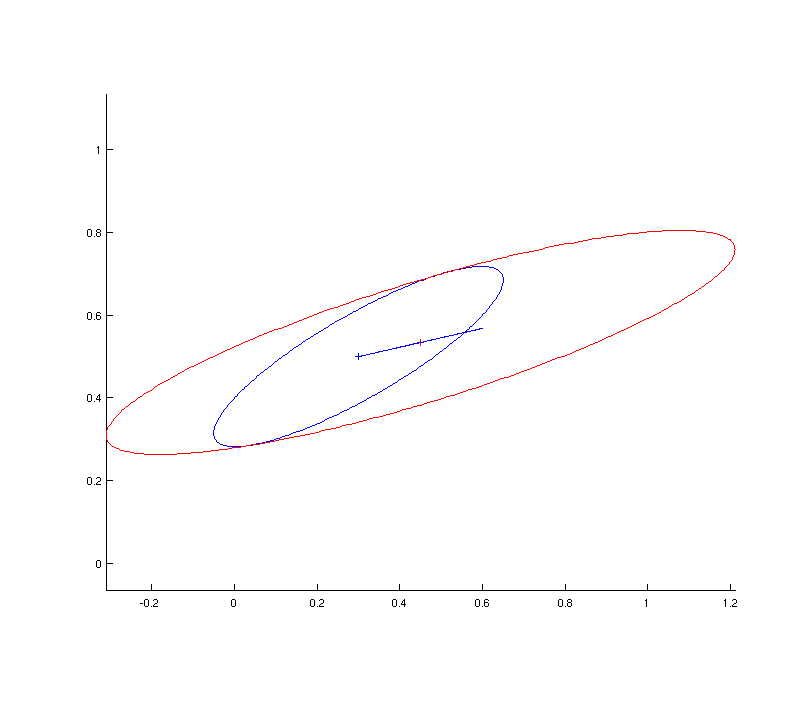
\includegraphics[width=0.4\textwidth]{figures/alpha2d-95.png}}
    \caption{\it 1-$\sigma$ contour ellipse for estimate $(\v{m}_1,\m{M}_1)$ and the mean shift term
        $(\v{u}-\v{m}_1)(\v{u}-\v{m}_1)'$ (blue), together with the intermediate covariance 1-$\sigma$ ellipse (red),
        for example \ref{ex:gcu2d}.}
    \label{fig:alpha2d}
\end{figure}
Figure \ref{fig:alpha2d} shows the 1-$\sigma$ contour ellipse of $(\v{m}_1,\m{M}_1)$ and
$\left(\v{u},\frac{\m{M}_1}{\alpha_1}+\frac{(\v{u}-\v{m}_1)(\v{u}-\v{m}_1)'}{1-\alpha_1}\right)$ for different values of
$\alpha_1$. The input $(\v{m}_1,\m{M}_1)$ is given. The mean shift term $(\v{u}-\v{m}_1)(\v{u}-\v{m}_1)'$ is a
single-component matrix which forms an ellipse with major axis twice the length of the shift, and minor axis of
length zero, centered at $\v{u}$ and aligned with both means. The intermediate covariance is a linear sum of these two
components, with the interpolation between $\alpha_1=0$ and $\alpha_1=1$ creating an unbounded asymptotic behavior which
is roughly similar to that shown in figure \ref{fig:alpha1dcurve} in the 1-D case. The 1-$\sigma$ ellipse given by
$\tau_1(\alpha_1=0)$ will be infinite in size, with the same shape as $\varepsilon_1$; at the other end,
$\tau_1(\alpha_1=1)$ will be infinite in length, with the same orientation as the mean shift term and the exact width of
the projection of $\varepsilon_1$ in the orthogonal direction.

By choosing values for $\alpha_1$ it is possible to compare $\tau_1(\alpha_1)$ with $\varepsilon_1$ and test for
containment and confirm that $\varepsilon_1$ is always completely contained. Taking $\alpha_1=0.75$, $\tau_1$ becomes
\begin{equation}
    \tau_1(\alpha_1=0.75)=\left\{
        \begin{aligned}
            A_{\tau,1} &=
            \left[\begin{smallmatrix}
                 11.8286 & -18.6285\\
                -18.6285 &  44.0408
            \end{smallmatrix}\right]\\
            b_{\tau,1} &=
            \left[\begin{smallmatrix}
                  4.6295\\
                -15.1454
            \end{smallmatrix}\right]\\
            c_{\tau,1} &=  \begin{smallmatrix}6.0078\end{smallmatrix}
        \end{aligned}\right.
\end{equation}
and the solution to $\lambda_{max}$ described in section \ref{section:containment} is $-0.0696$, so the condition
$\lambda_{max}\leq 0$ for $\tau_1$ to properly contain $\varepsilon_1$~\cite{eberly00}, holds.


\end{example}


% ND, projections
\section{Extension to Higher Dimensions}


It becomes increasingly difficult to visualize any of the covariance or ellipsoid components as the dimensionality
increases. For example, in three dimensions, the 1-$\sigma$ contour ellipsoid is a three-dimensional cross-section of a
four-dimensional Gaussian volume, which is rotated by both an elevation angle $\phi$ and an azimuth angle
$\theta$. However, even in these higher state spaces, the mathematics operate in the same fashion as described for the
one- and two-dimensional cases.

One rough method to check a higher-dimensional GCU result for ellipsoid enclosure (although not strictly {\em minimal}
enclosure) is to project the set of $n$-dimensional ellipsoids into all possible two-dimensional major axis component
planes. Properly contained ellipsoids should still be properly contained in any lower-dimensional projection. Figure
\ref{fig:cu3d} illustrates this property by projecting a set of three-dimensional 1-$\sigma$ contour ellipsoids into the
$xy$, $xz$, and $yz$ planes.
\begin{figure}[tbp]
    \centering
        \subfloat[Projection into $xy$ plane]{\label{fig:cu3dxy}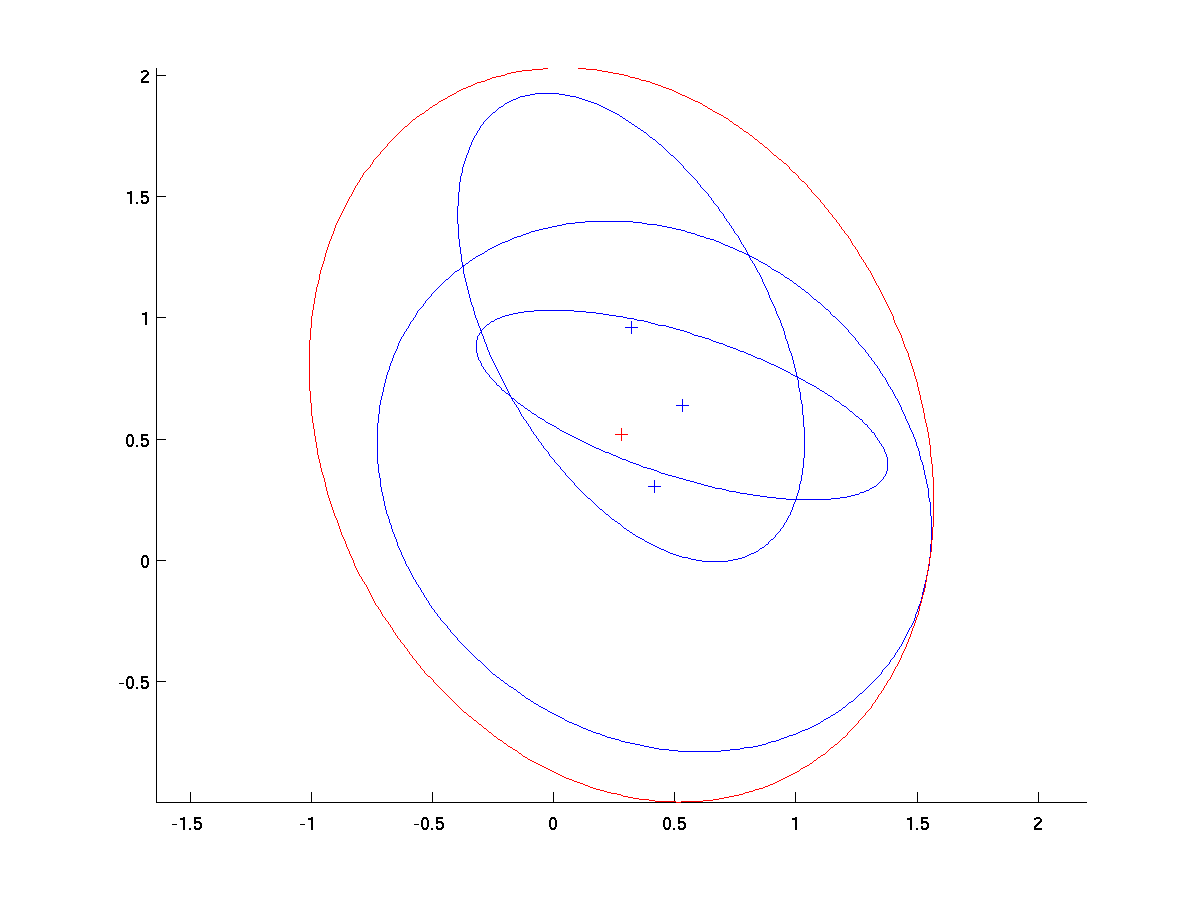
\includegraphics[width=0.4\textwidth]{figures/cu3dxy.png}}
        \subfloat[Projection into $xz$ plane]{\label{fig:cu3dxz}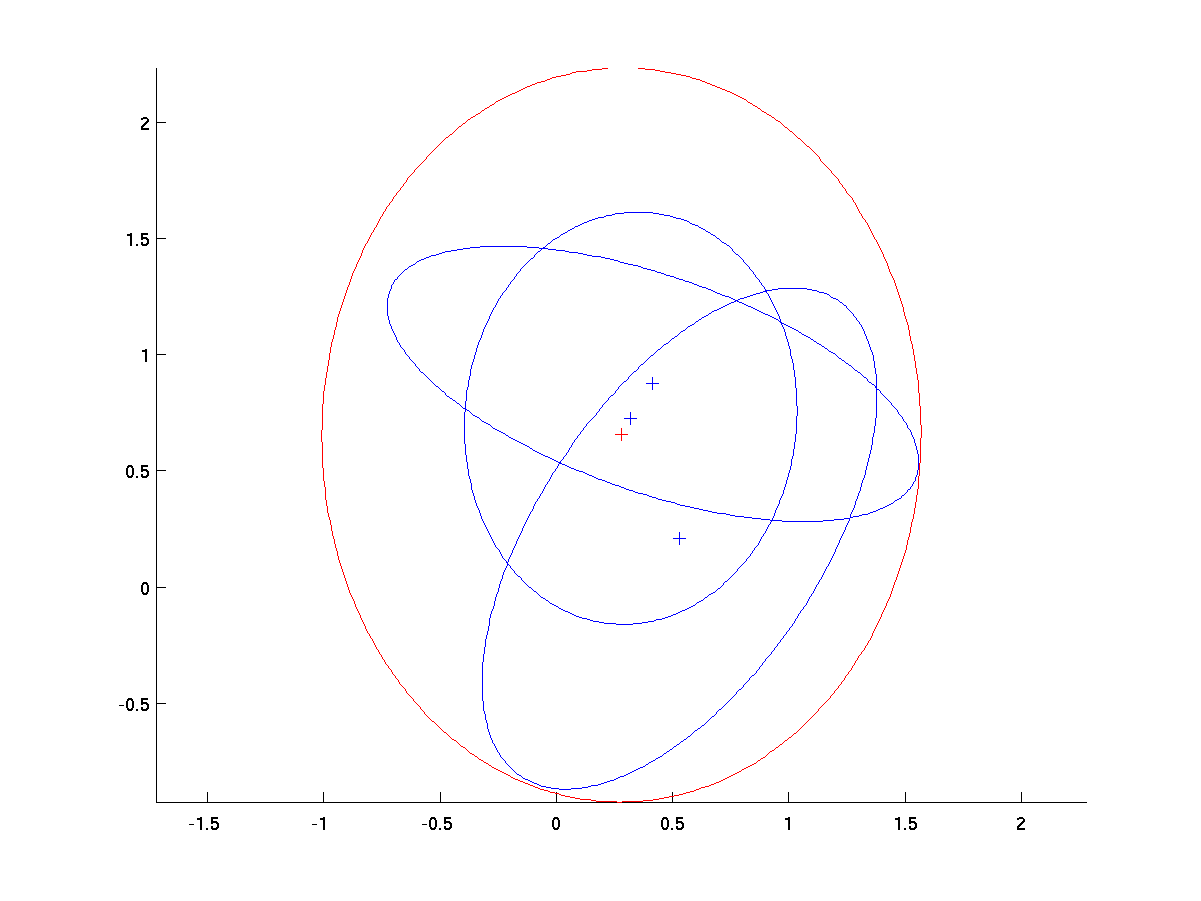
\includegraphics[width=0.4\textwidth]{figures/cu3dxz.png}}

        \subfloat[Projection into $yz$ plane]{\label{fig:cu3dyz}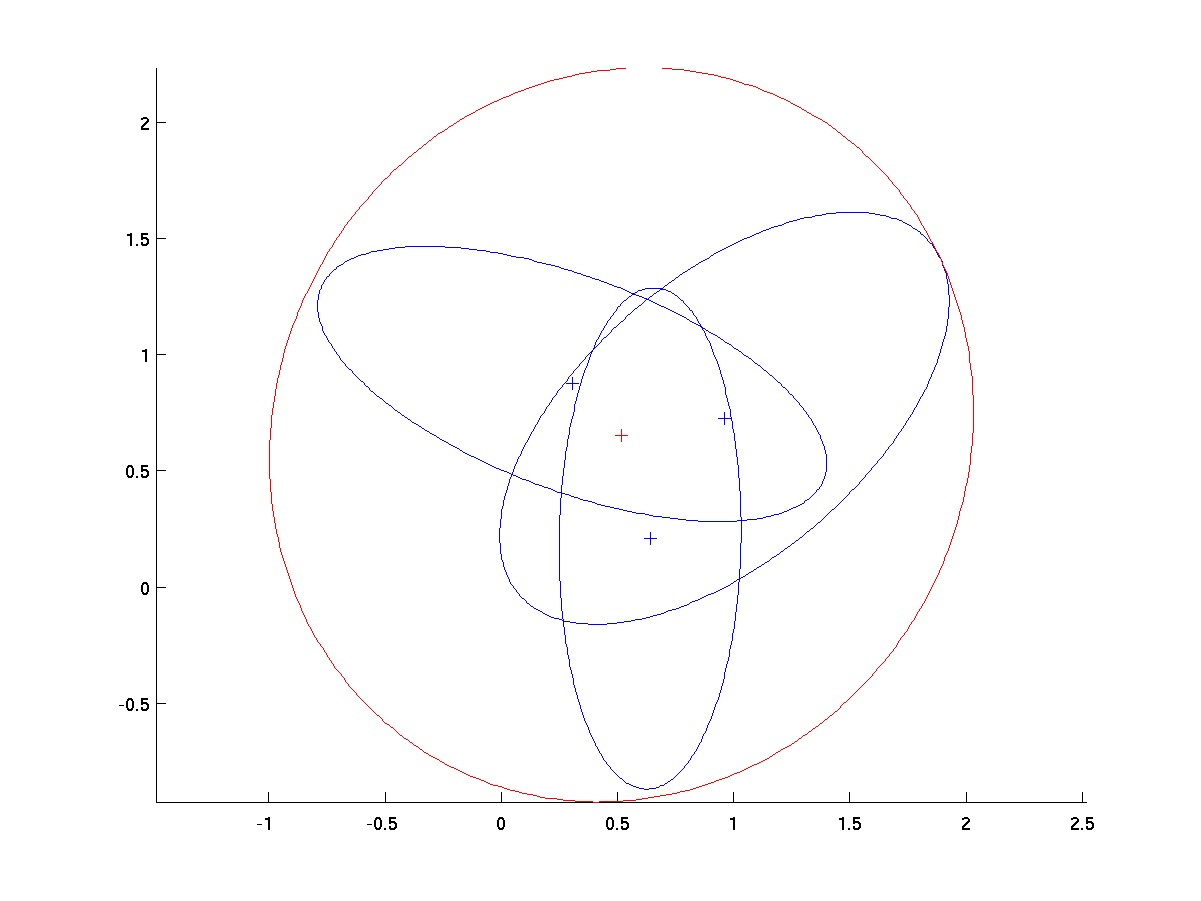
\includegraphics[width=0.4\textwidth]{figures/cu3dyz.png}}
    \caption{\it 1-$\sigma$ contour plots of three 3D input estimates (blue) together with the batch GCU result (red),
        projected down into the three 2D major axis component planes. }
    \label{fig:cu3d}
\end{figure}
Computation of the sixth-order $P(t)$ polynomial (equation \ref{eqn:poly}) for the Lagrange test confirms that the GCU
result 1-$\sigma$ contour ellipsoid properly contains its inputs in three-dimensional space as well, the space in which
this result is known to be minimized.


% Additional 2D figures
\section{Additional Examples}\label{section:examples}

In this section, further examples of two-dimensional GCU are plotted as 1-$\sigma$ contour ellipses to provide further
evidence that a GCU solution satisfies the MEEE requirements. The procedure used for each example is:
\begin{enumerate}
    \item Randomly generate five mean and covariance estimates, $(\v{m}_i,\m{M}_i)$, $i=1\dots 5$.
    \item Calculate $(\v{u},\m{U})$ as the batch GCU of $(\v{m}_i,\m{M}_i)$, $i=1\dots 5$.
    \item Use the transformation in equation \ref{eqn:cu2e} to find the ellipses $\varepsilon_0=\mathbb{T}(\v{u},\m{U})$
        and $\varepsilon_i=\mathbb{T}(\v{m}_i,\m{M}_i)$, $i=1\dots 5$.
    \item Use the procedure in section \ref{section:containment} to find $\lambda_{max}$ for each $Q_0$ and $Q_i$,
        $i=1\dots 5$.
\end{enumerate}
The fives values of $\lambda_{max}\leq 0$ are given as numerical results to support the claim that each GCU ellipse
actually does properly contain all of its inputs~\cite{eberly00}. The 1-$\sigma$ contour plots are shown in figure
\ref{fig:cu2d-5}, and the numerical values of $\lambda_{max}$ are listed in table \ref{tab:cu2d-5}.

\begin{figure}[tbp]
    \centering
        \subfloat[]{\label{fig:cu2d-5a}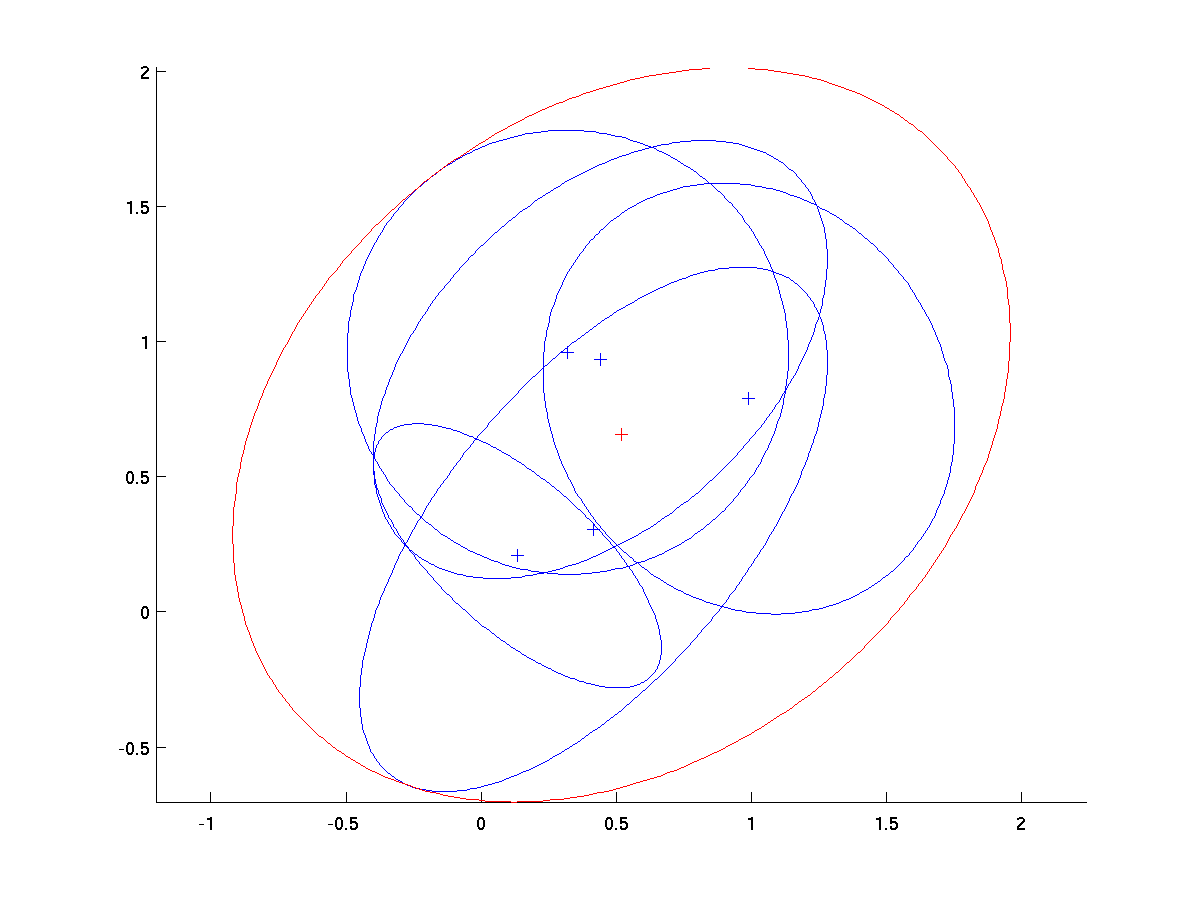
\includegraphics[width=0.4\textwidth]{figures/cu2d-5a.png}}
        \subfloat[]{\label{fig:cu2d-5b}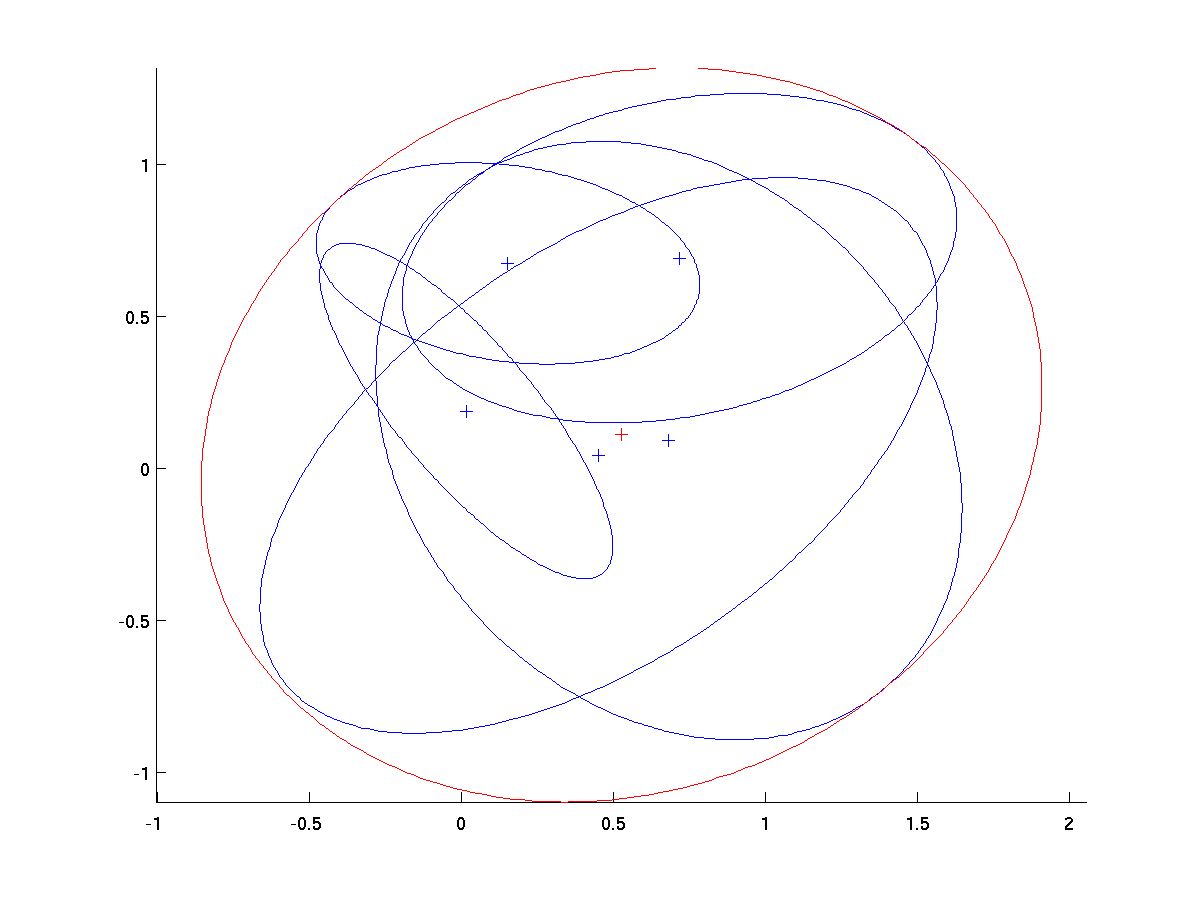
\includegraphics[width=0.4\textwidth]{figures/cu2d-5b.png}}

        \subfloat[]{\label{fig:cu2d-5c}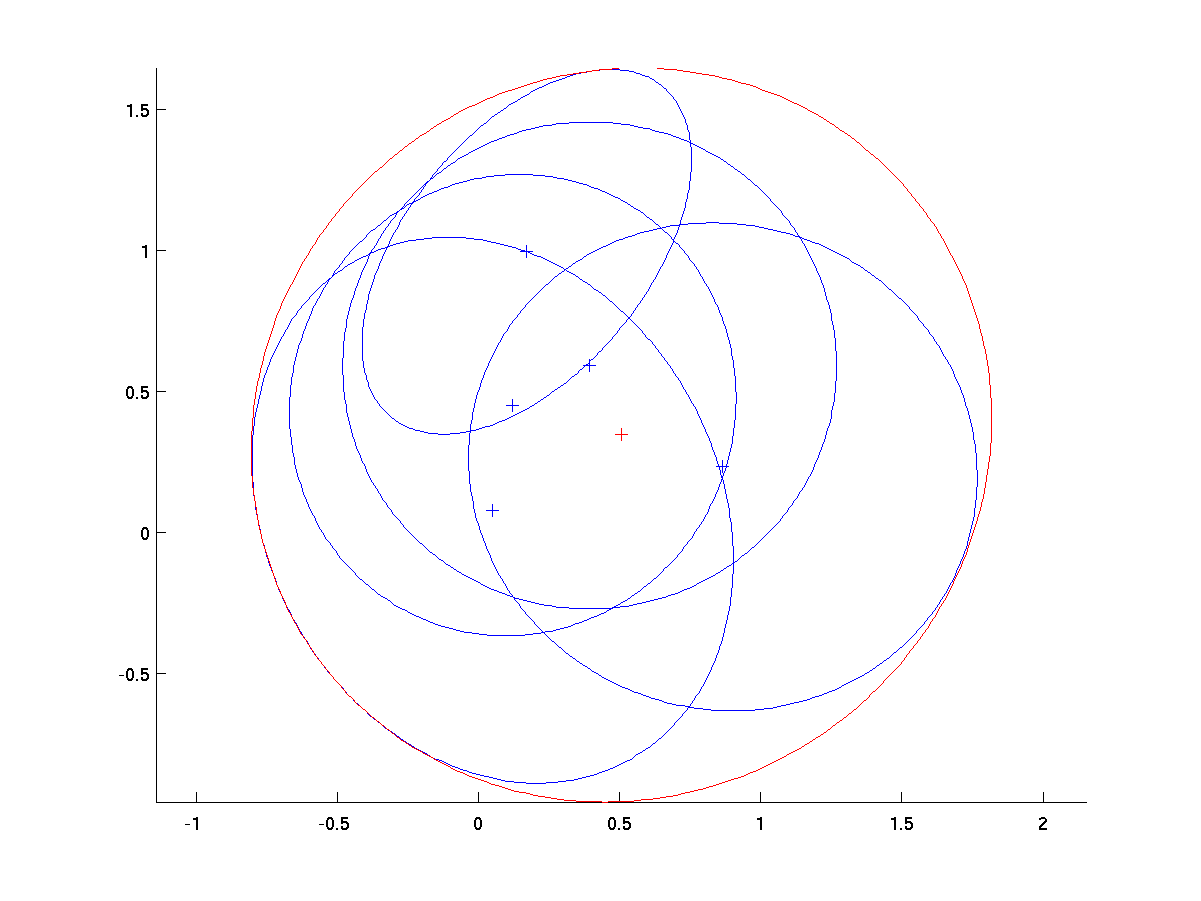
\includegraphics[width=0.4\textwidth]{figures/cu2d-5c.png}}
        \subfloat[]{\label{fig:cu2d-5d}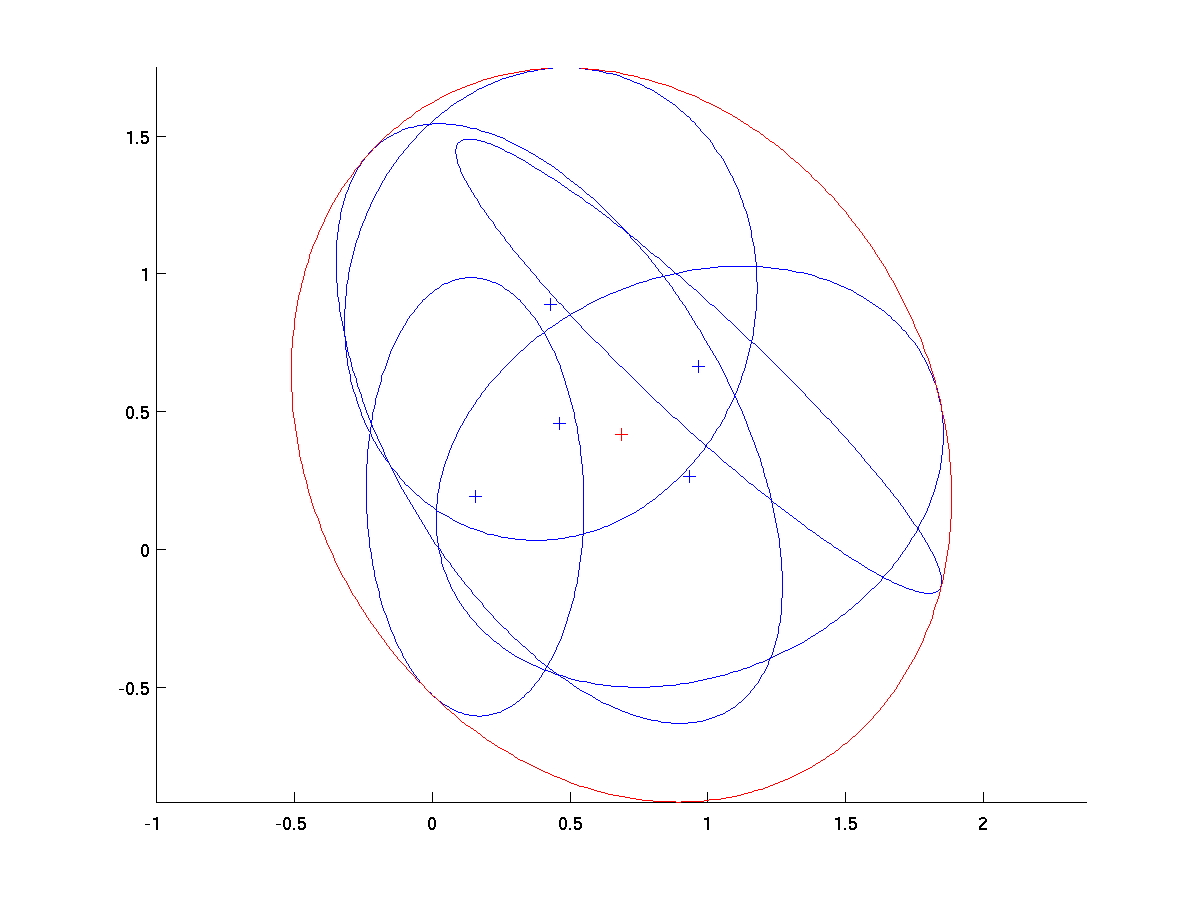
\includegraphics[width=0.4\textwidth]{figures/cu2d-5d.png}}

        \subfloat[]{\label{fig:cu2d-5e}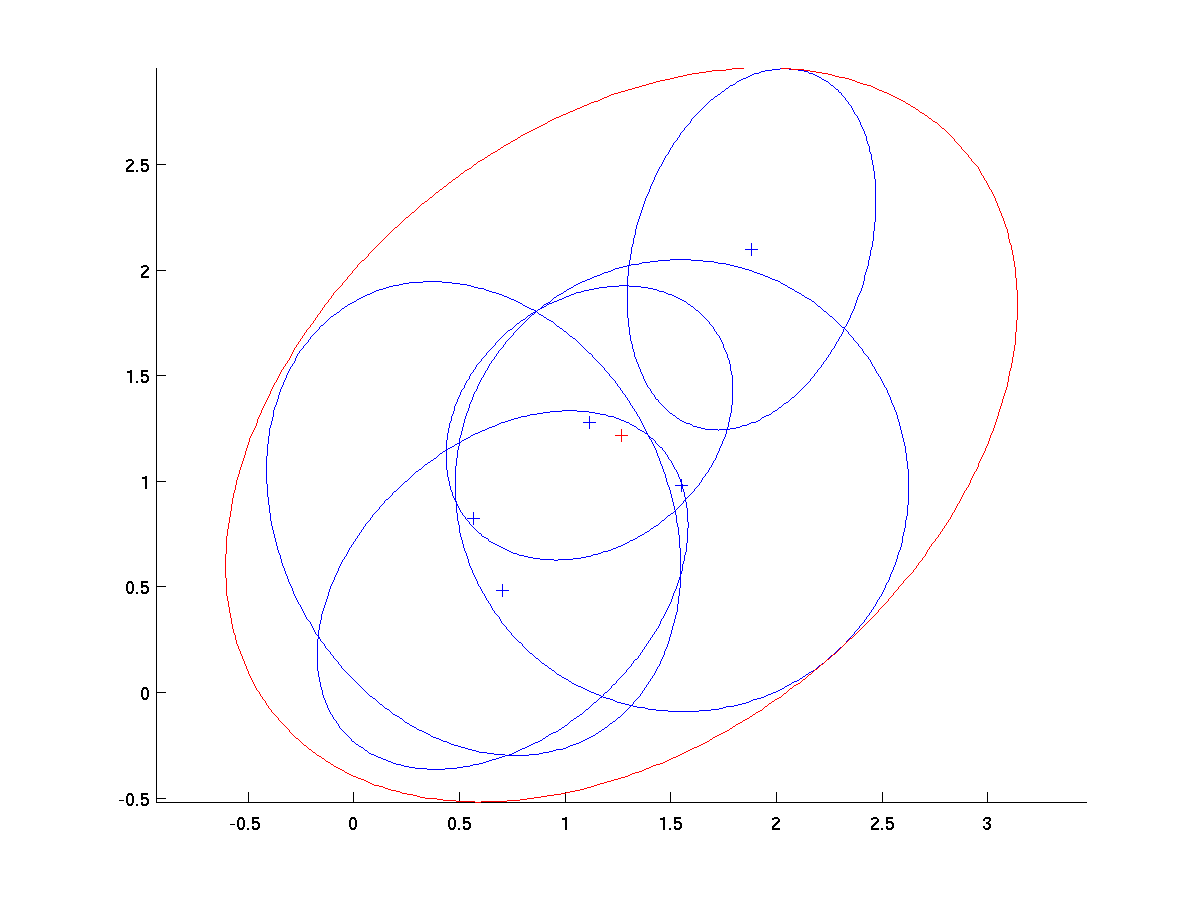
\includegraphics[width=0.4\textwidth]{figures/cu2d-5e.png}}
        \subfloat[]{\label{fig:cu2d-5f}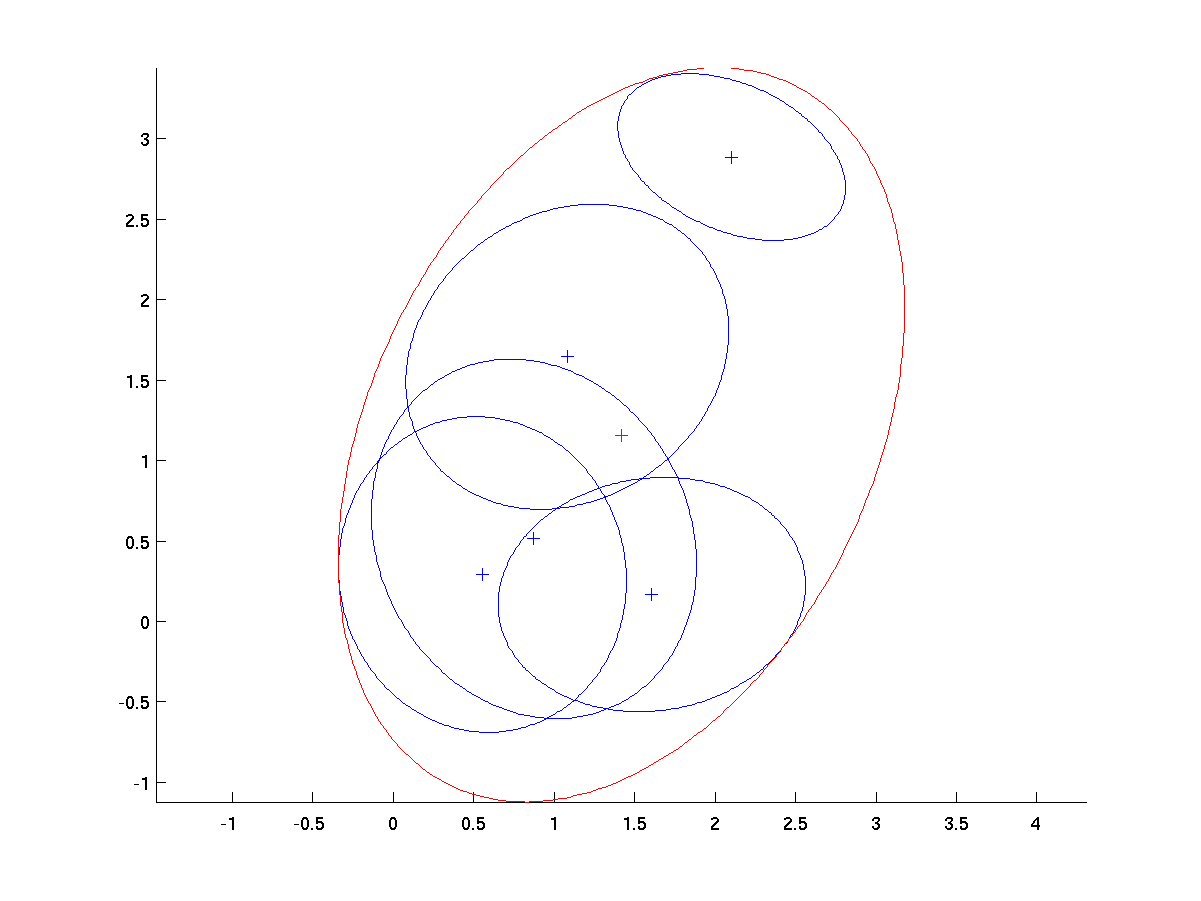
\includegraphics[width=0.4\textwidth]{figures/cu2d-5f.png}}
    \caption{\it 1-$\sigma$ contour plots of five 2D input estimates (blue) together with the batch GCU result (red). Figures
        (a) through (f) are independent examples, and the numerical results for
        $\lambda_{max}$ are given in table \ref{tab:cu2d-5}. }
    \label{fig:cu2d-5}
\end{figure}

\begin{table}
\centering
\begin{tabular*}{0.8\textwidth}{@{\extracolsep{\fill}}r@{.}lr@{.}lr@{.}lr@{.}lr@{.}lr@{.}l}
\multicolumn{2}{c}{Ex. (a)} &
\multicolumn{2}{c}{Ex. (b)} &
\multicolumn{2}{c}{Ex. (c)} &
\multicolumn{2}{c}{Ex. (d)} &
\multicolumn{2}{c}{Ex. (e)} &
\multicolumn{2}{c}{Ex. (f)}\\
\hline
-1&40e-4    &  -0&0264      &  -0&1592  &  -2&24e-5 &  -6&64e-5 &  -0&1353 \\
-0&1374     &  -2&31e-5     &  -0&0095  &  -9&24e-4 &  -0&7482  &  -0&0078 \\
-1&99e-5    &  -0&1508      &  -3&96e-5 &  -4&44e-5 &  -1&51e-4 &  -1&64e-4 \\
-0&3566     &  -1&21e-4     &  -5&16e-5 &  -1&53e-5 &  -0&1234  &  -0&2035 \\
-0&4794     &  -1&79e-4     &  -0&2109  &  -1&19e-5 &  -0&0356  &  -1&72e-5\\
\end{tabular*}
    \caption{\it Five $\lambda_{max}$ values for the six GCU trials shown in figure \ref{fig:cu2d-5}. Note that all of these
        values satisfy the condition $\lambda_{max}\leq 0$ to show that the GCU 1-$\sigma$ contour ellipse properly contains its 
        five inputs. } 
    \label{tab:cu2d-5}
\end{table}




